\subsection{Option Prices}\label{sec:option-prices}

The price paths were generated with the ForGAN baseline model under configuration 8, selected in Sec.~\ref{sec:model-selection}, and priced through the procedure described in Sec.~\ref{sec:pricing-setup}. The generated option prices are evaluated against the market prices as well as the benchmarks of Sec.~\ref{sec:benchmarks}. Option prices depend on the distance between the strike and the settlement price on the valuation date, so prices at different strikes are not comparable. The models are compared through the implied volatility. The error of a strike is the absolute difference between the two implied volatilities,
\begin{equation}
    e_{d,k} = \left| \hat{\sigma}_{d,k} - \sigma_{d,k} \right|,
    \label{eq:strike-error}
\end{equation}
where $\hat{\sigma}_{d,k}$ is the implied volatility of the simulated price for strike $k$ on valuation date $d$, and $\sigma_{d,k}$ is the implied volatility published by the exchange. The error of a model is the mean of the $e_{d,k}$ of a valuation date, averaged over \num{20} valuation dates,
\begin{equation}
    e = \frac{1}{20} \sum_{d=1}^{20} \frac{1}{n_d} \sum_{k=1}^{n_d} e_{d,k},
    \label{eq:model-error}
\end{equation}
where $n_d$ is the number of strikes with an implied volatility on valuation date $d$. Every valuation date carries the same weight, independently of the number of strikes. The strikes with no implied volatility are excluded from both errors, and the percentage of inverted strikes is reported alongside. The signed error $s$ is Eq.~\eqref{eq:model-error} computed without the absolute value of Eq.~\eqref{eq:strike-error}. The error measures the size of the deviation from the market, and the signed error its direction. The results are reported in Tab.~\ref{tab:price-error}. $G$ was priced with each of the five seeds separately and is reported as mean and seed spread. The benchmarks carry a single seed each (Sec.~\ref{sec:benchmarks}).

The block bootstrap has the lowest $e$ at \num{0.123}, followed by the $\mathrm{iid}$ bootstrap at \num{0.141} and GBM at \num{0.154}. The prices generated by $G$ have the highest $e$ at \num{0.255}, with a seed spread of \num{0.041}. The seed range does not overlap with any of the benchmarks. The signed error is negative for all models. For the block bootstrap it is \num{-0.006}, so the deviations are of both signs and cancel each other out. The signed error of $G$ is \msa{-0.228}{0.053}, and negative on every seed, so the generated prices lie below the market. $G$ also inverts the fewest strikes, at \SI{79.8}{\percent} against \SI{100}{\percent} for both bootstrap modes.

\begin{table}[htbp]
  \centering
  \begin{tabular}{lrrr}
    \toprule
    Model & $e$ & $s$ & Inverted (\si{\percent}) \\
    \midrule
    GBM & 0.154 & $-0.130$ & 88.9 \\
    Bootstrap, $\mathrm{iid}$  & 0.141 & $-0.087$ & 100.0 \\
    Bootstrap, block          & 0.123 & $-0.006$ & 100.0 \\
    $G$                       & \msa{0.255}{0.041} & \msa{-0.228}{0.053} & \msa{79.8}{13.1} \\
    \bottomrule
  \end{tabular}
  \caption{Implied volatility error, signed error and percentage of inverted strikes}
  \label{tab:price-error}
\end{table}

The error of Tab.~\ref{tab:price-error} does not show where the model deviates from the market across different strikes, since it is aggregated over all strikes. The strikes were grouped into four ranges of moneyness within the band of Sec.~\ref{sec:options-data}, and $e$ was computed within each range. The in-the-money strikes cover moneyness \numrange{0.5}{0.9} and the at-the-money strikes \numrange{0.9}{1.1}. The out-of-the-money strikes cover moneyness \numrange{1.1}{2.0} and were split at \num{1.5}, since the range is wider than the other two. The results are reported in Tab.~\ref{tab:price-error-moneyness}.

\begin{table}[htbp]
  \centering
  \begin{tabular}{lrrrr}
    \toprule
    Model & \numrange{0.5}{0.9} & \numrange{0.9}{1.1} & \numrange{1.1}{1.5} & \numrange{1.5}{2.0} \\
    \midrule
    GBM & 0.148 & 0.019 & 0.155 & 0.325 \\
    Bootstrap, $\mathrm{iid}$            & 0.107 & 0.154 & 0.142 & 0.208 \\
    Bootstrap, block          & 0.082 & 0.144 & 0.151 & 0.154 \\
    $G$ & \msa{0.257}{0.115} & \msa{0.243}{0.061} & \msa{0.309}{0.070} & \msa{0.341}{0.111} \\
    \bottomrule
  \end{tabular}
  \caption{Implied volatility error by moneyness}
  \label{tab:price-error-moneyness}
\end{table}

GBM has the lowest error for at-the-money strikes, at \num{0.019}. The implied volatility used to price GBM is the listed implied volatility at the strike closest to the settlement price on the valuation date (Sec.~\ref{sec:benchmarks}). As a result, the at-the-money strikes match the market by construction and the value does not measure the accuracy of the model. The in-the-money strikes have an error of \num{0.148}, the out-of-the-money strikes \num{0.155}, and the far out-of-the-money strikes \num{0.325}. A single $\sigma$ produces the same implied volatility at every strike, while the market implied volatility varies across strikes. The error of the block bootstrap ranges between \num{0.082} for the in-the-money strikes and \num{0.154} for the far out-of-the-money strikes. The $\mathrm{iid}$ bootstrap has a higher error for the far out-of-the-money strikes, at \num{0.208}. The order of returns is the only difference between the two bootstrap modes (Sec.~\ref{sec:benchmarks}), so the gap reflects the volatility clustering.

$G$ has the highest error in every range, \num{0.243} for at-the-money strikes to \num{0.341} far out-of-the-money strikes. The at-the-money error is higher than the \num{0.144} of the block bootstrap. The prices at the at-the-money strikes do not depend on the extreme returns, so the deviation is not caused by the tail weight alone. The results of $G$ by moneyness are reported in more detail in Tab.~\ref{tab:price-error-generator}.

\begin{table}[htbp]
  \centering
  \begin{tabular}{lrrr}
    \toprule
    Moneyness & $e$ & $s$ & Inverted \\
    \midrule
    \numrange{0.5}{0.9} & \msa{0.257}{0.115} & \msa{-0.236}{0.135} & \msa{82.6}{17.4} \\
    \numrange{0.9}{1.1} & \msa{0.243}{0.061} & \msa{-0.213}{0.090} & \msa{100.0}{0.0} \\
    \numrange{1.1}{1.5} & \msa{0.309}{0.070} & \msa{-0.288}{0.089} & \msa{91.9}{13.8} \\
    \numrange{1.5}{2.0} & \msa{0.341}{0.111} & \msa{-0.306}{0.162} & \msa{53.8}{43.3} \\
    \bottomrule
  \end{tabular}
  \caption{Implied volatility error, signed error and percentage of
           inverted strikes of $G$ by moneyness}
  \label{tab:price-error-generator}
\end{table}

The signed error is negative in every range, so the generated prices lie below the market prices in all moneyness ranges. The percentage of inverted strikes falls with the distance from the at-the-money strikes, from \SI{100}{\percent} at the money to \SI{53.8}{\percent} far out of the money. The seed spread of the far out-of-the-money strikes is \num{43.3}, close to the mean of \num{53.8}. The seeds differ in whether the simulated paths reach the outer strikes at all. The excluded strikes are those no simulated path reaches, so the reported error is smaller than the true deviation. The same holds for GBM.

The errors of Tab.~\ref{tab:price-error-moneyness} are averaged over the \num{20} valuation dates and do not show the shape of the deviation on a single date. Three valuation dates are reported in Fig.~\ref{fig:vol-smile-models}, covering the range of market conditions in the test split. 2025-10-28 has the lowest implied volatility at the at-the-money strike, at \num{0.316}, and 2026-03-25 the highest, at \num{1.132}. 2025-01-24 lies between them at \num{0.528}. The curve of $G$ is the mean across the seeds. The shaded area covers the range of the five seeds at each strike. The curves end where the inversion fails.

\begin{figure}[htbp]
    \centering
    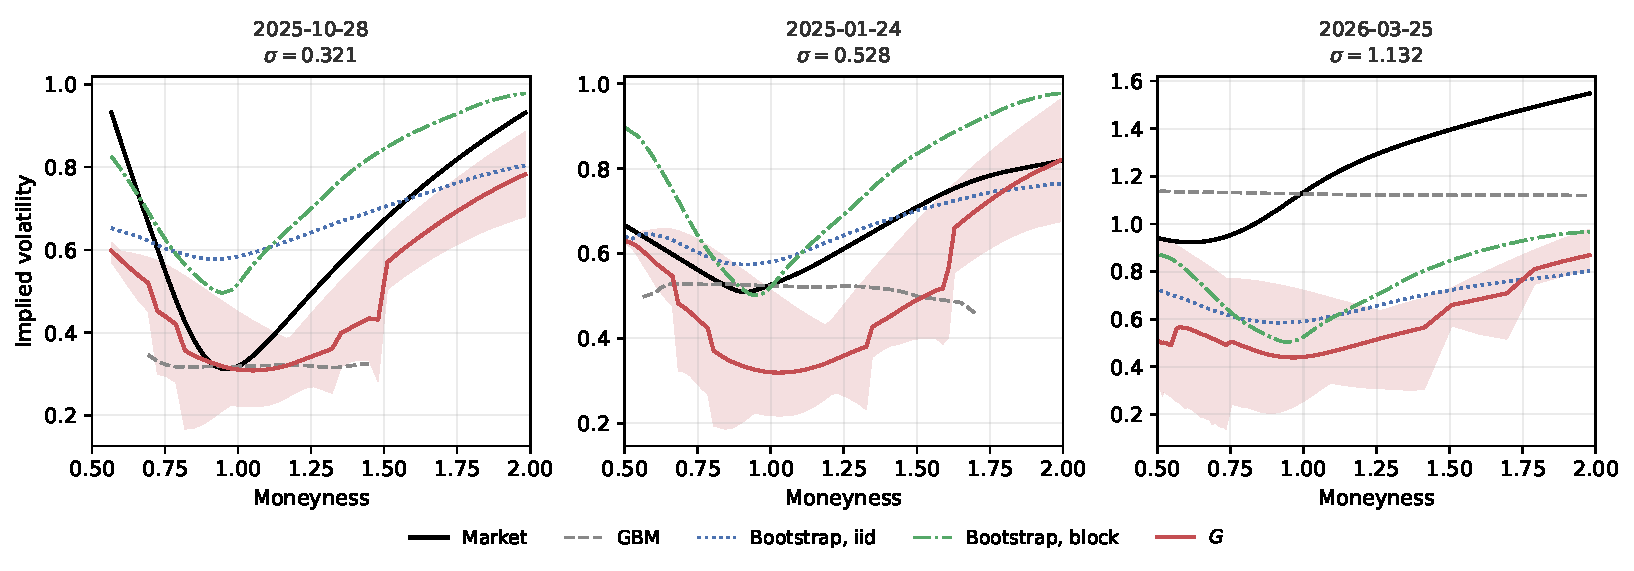
\includegraphics[width=\textwidth]{figures/smiles.pdf}
    \caption{Implied volatility against moneyness on three valuation dates}
    \label{fig:vol-smile-models}
\end{figure}

The market implied volatility is a smile on all three valuation dates. GBM produces a flat implied volatility, since a single $\sigma$ applies to
every strike. Both bootstrap modes overprice the options on the first two valuation dates. The block mode captures the shape of the market, while the $\mathrm{iid}$ mode produces a flatter smile. The implied volatility of $G$ lies below the market on all three dates. 

The third date falls in the 2026 disruption described in Sec.~\ref{sec:gas-markets}. The market implied volatility rises from \num{0.92} for the at-the-money strike to \num{1.55} for the far out-of-the-money strike. Both bootstrap modes and $G$ stay below \num{1.0}. The bootstrap draws from the same training split on every valuation date (Sec.~\ref{sec:benchmarks}), so the simulated distribution does not change with the market conditions. GBM matches the market at the at-the-money strike, since its $\sigma$ is taken from there. $G$ is conditioned on the returns preceding the valuation date. The annualized spread of the simulated \num{20}-day return of $G$ and the block bootstrap is reported in Fig.~\ref{fig:conditioning}, together with the implied volatility at the at-the-money strike.

\begin{figure}[htbp]
    \centering
    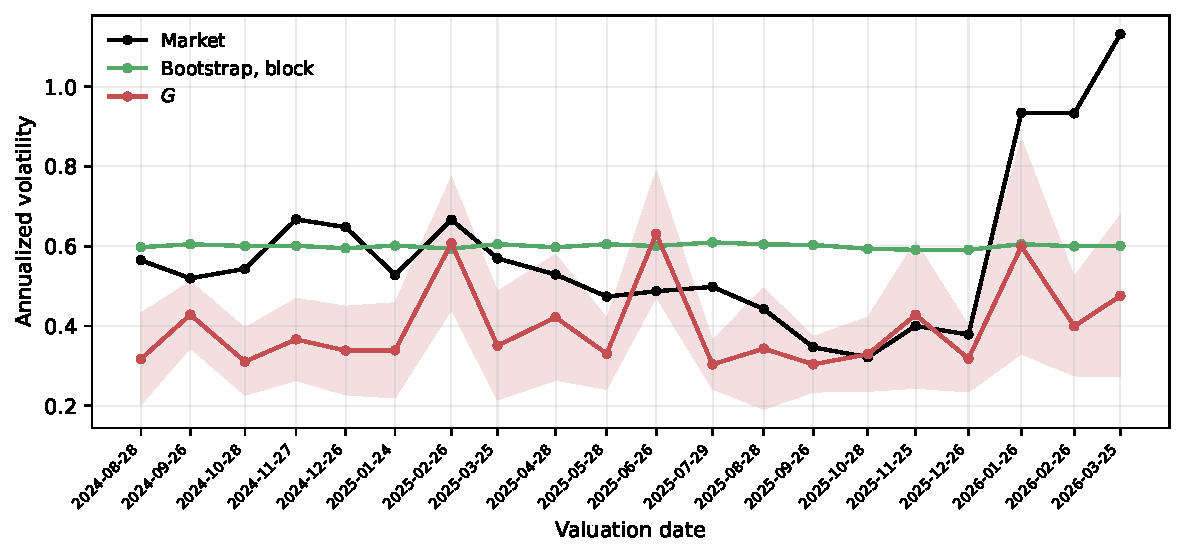
\includegraphics[width=\textwidth]{figures/conditioning.pdf}
    \caption{Annualized volatility on each valuation date}
    \label{fig:conditioning}
\end{figure}

The spread of the block bootstrap ranges from \num{0.588} to \num{0.608}. The spread of $G$ ranges from \num{0.300} to \num{0.615}, and its correlation with the spread of the realized returns in the condition window is \num{0.752}. The simulated distribution of $G$ widens when the preceding returns are turbulent. As a result, the conditioning of $G$ produces a response. The spread of $G$ is below the implied volatility of the market on \num{17} of the \num{20} valuation dates, so the response does not reach the level of the market.

The reported results of $G$ were generated with the ForGAN baseline cost function. The $\mathrm{PnL}^{*}_{a}$ and $\mathrm{PnL}^{*}_{a}$ \& $\mathrm{MSE}$ branches closest to the test split were priced as well (Sec.~\ref{sec:effect-cost}). The results are reported in Tab.~\ref{tab:price-error-branches}. The error of the ForGAN baseline is the lowest among the three cost function branches. The seed spread of the ForGAN baseline is the smallest at \num{0.041} against \num{0.369} for the $\mathrm{PnL}^{*}_{a}$ branch. The signed error of the $\mathrm{PnL}^{*}_{a}$ branch is \num{0.023} with a seed spread of \num{0.508}, so some seeds price above the market and others below. Compared with the ForGAN baseline, the seed spread of the $\mathrm{PnL}^{*}_{a}$ \& $\mathrm{MSE}$ branch is narrower on most of the generated return statistics (Sec.~\ref{sec:effect-cost}) and wider on the option prices.
The seed spread is not explained by the excess kurtosis of the generated returns. In the $\mathrm{PnL}^{*}_{a}$ branch, seed \num{2} has the highest excess kurtosis at \num{21.59} and an error of \num{0.303}, close to the errors of the other seeds. In contrast, seed \num{4} has the largest error of \num{1.101} with an excess kurtosis of \num{11.15}. As a result, the divergence arises in the recursive rollout of the generated returns (Sec.~\ref{sec:pricing-setup}), and not in the one-step distribution

\begin{table}[htbp]
  \centering
  \begin{tabular}{llrrrr}
    \toprule
    Cost function & Seed & Kurtosis & $e$ & $s$ & Inverted (\si{\percent}) \\
    \midrule
    ForGAN & 0 & 13.24 & 0.199 & $-0.163$ & 74.9 \\
           & 1 &  7.61 & 0.237 & $-0.214$ & 96.2 \\
           & 2 & 12.46 & 0.308 & $-0.287$ & 79.1 \\
           & 3 &  9.38 & 0.251 & $-0.200$ & 87.4 \\
           & 4 &  7.93 & 0.279 & $-0.278$ & 61.4 \\
    \addlinespace
    $\mathrm{PnL}^{*}_{a}$ & 0 & 10.12 & 0.193 & $-0.168$ & 92.4 \\
           & 1 &  8.40 & 0.366 & $-0.047$ & 89.3 \\
           & 2 & 21.59 & 0.303 & $-0.303$ & 80.9 \\
           & 3 &  8.90 & 0.284 & $-0.281$ & 83.0 \\
           & 4 & 11.15 & 1.101 & \phantom{$-$}0.912 & 79.0 \\
    \addlinespace
    $\mathrm{PnL}^{*}_{a}$ \& $\mathrm{MSE}$ & 0 & 11.62 & 0.208 & $-0.160$ & 92.2 \\
           & 1 & 11.88 & 0.320 & $-0.313$ & 73.5 \\
           & 2 & 12.30 & 0.230 & $-0.222$ & 93.9 \\
           & 3 &  5.39 & 0.271 & $-0.241$ & 80.4 \\
           & 4 & 12.23 & 0.549 & \phantom{$-$}0.190 & 86.2 \\
    \bottomrule
  \end{tabular}
  \caption{Excess kurtosis of the generated returns and option pricing
           results per seed, configuration 8}
  \label{tab:price-error-branches}
\end{table}

The prices generated by $G$ deviate further from the market than the prices of the benchmarks in every moneyness range. The deviation is a systematic underpricing, and $G$ reaches the fewest strikes. However, $G$ is the only model that responds to the state of the market at the valuation date, although the response does not reach the level of the market.